\documentclass[12pt]{article} % The document class with options

\usepackage[margin=1in]{geometry}
\usepackage[utf8]{inputenc} 
\geometry{a4paper}
\usepackage{newtxtext,newtxmath}
\usepackage[T1]{fontenc}
\usepackage{amsmath}
\usepackage{amsfonts}
\usepackage{microtype}
\usepackage{graphicx}
\usepackage{listings} % For formatting and highlighting code
\usepackage{color}    % For colors in code highlighting

% chktex-file 3
% chktex-file 8
% chktex-file 10
% chktex-file 17
% chktex-file 18
% chktex-file 36
% chktex-file 44

\begin{document}
\setlength{\parskip}{1em} 
\setlength{\parindent}{0pt}
\newcommand{\vect}[1]{\mathbf{#1}}

\begin{titlepage}  % This starts a title page environment
    \centering    % Center everything on the page

    %--- Add space at the top of the page ---
    \vspace*{2cm}
    
    %--- Title ---
    \normalsize \textbf{MEng Project Report} \\
    \vspace{0.5cm}  % Space between lines
    \normalsize\textbf{Model Analysis of DTMB5415 and BURNSI Ship Model} \\
    \vspace{2cm}  % Space between the title and the author name
    
    %--- Author ---
    \normalsize by\\
    \vspace{1cm}
    \normalsize Jincong Li \\ 
    \vspace{1cm}
    \normalsize M.Eng, The University of British Columbia, 2024
    \vspace{11cm}  % Space between the author and the date
    
    %--- Date ---
    \normalsize \today

    \vfill  % Push the following content to the bottom of the page
    %--- Bottom part of the page ---
    © Jincong Li, 2024
\end{titlepage}
\tableofcontents
\newpage
\section{Abstract}

\section{Introduction}
This project investigated into the global response of BURNSi ship model under the influence of surface waves.

\subsection{DTMB5415}

The ship model used for the first part of this project is DTMB5415, which was conceived as a preliminary design for a Navy surface combatant around 1980. The hull geometry of Model 5415 includes both a sonar dome and a transom stern. Propulsion is provided through twin open-water propellers driven by shafts supported by struts.

It is important to note that no full-scale ship exists for this model. The hull geometry and relevant loading conditions and speeds are detailed in the Appendix section.
\begin{figure}[ht]
    \centering
    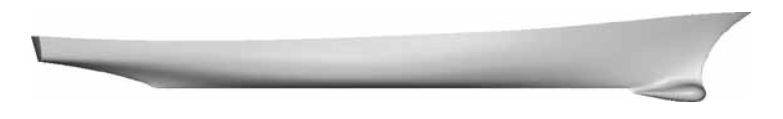
\includegraphics[width=1\textwidth]{DTMB.png}
    \caption{Side of DTMB5415}
\end{figure}


\subsection{BURNSI Ship Model}

The BURNSi ship model is part of a project aimed at benchmarking and validating numerical prediction tools for underwater radiated noise (URN) levels. The model represents an ORCA-class training vessel of the Royal Canadian Navy. Key specifications of the vessel include:

\begin{itemize}
    \item \textbf{Displacement:} 210 Tonnes
    \item \textbf{Length:} 33 meters
    \item \textbf{Beam:} 8.3 meters
    \item \textbf{Keel depth:} 2 meters
    \item \textbf{Hull material:} Steel
    \item \textbf{Propulsion:} 2 x 1864 KW Diesel Engines
    \item \textbf{Maximum Speed:} 20 knots
\end{itemize}

The vessel is equipped with various machinery including 5-bladed fixed pitch propellers, propulsion diesel engines (CAT3516), diesel generator sets (CAT3054T), and other supporting systems such as air compressors and hydraulic power packs. The URN prediction involves assessing noise from sources like diesel generators, propulsion engines, gearboxes, and cavitation noise from propellers.


\section{Methodology}
The primary workflow of this project involves a two-step process. The initial step is to reproduce the results from Section 9.2 of Vaibhav Joshi's Ph.D. thesis \cite{joshi2018}. This section focuses on the analysis of the DTMB5415 ship model. The subsequent step is to replace the DTMB5415 ship model with the BURNSi ship model and conduct a similar model analysis.

The main target of this analysis is to study the heave motion of the BURNSi ship model under the same inlet wave conditions as those described in Section 9.2 of \cite{joshi2018}. By maintaining consistent wave conditions, we aim to directly compare the performance and characteristics of the BURNSi ship model against the baseline results obtained from the DTMB5415 ship model.

\begin{enumerate}
    \item \textbf{Reproduce Section 9.2 Results:}
    \begin{itemize}
        \item Follow the methodology outlined in Vaibhav Joshi's thesis to recreate the results using the DTMB5415 ship model.
        \item Validate the accuracy and consistency of the reproduced results with the original findings.
    \end{itemize}
    \item \textbf{Model Analysis with BURNSi Ship Model:}
    \begin{itemize}
        \item Replace the DTMB5415 ship model with the BURNSi ship model in the simulation framework.
        \item Conduct a detailed analysis focusing on the heave motion of the BURNSi ship model.
        \item Utilize the same inlet wave conditions as specified in Section 9.2 of \cite{joshi2018} to ensure comparability.
    \end{itemize}
\end{enumerate}

This approach allows for a systematic evaluation of the BURNSi ship model's performance in terms of its heave motion response, providing valuable insights for further improvements and applications.
%The main workflow of this project is first reproduce the result from section 9.2 of the Vaibhav's Ph.D thesis\cite{joshi2018}. 
%Then replace the DTMB5415 ship model with the BURNSi ship model to conduct a model analysis of that ship. The main target is the
%heave motion of the BURNSi ship model under the same inlet wave conditions as in the section 9.2 of\cite{joshi2018}.
\subsection{Mesh}
Note that for better view, only 2D mesh is presented below. A 3D view is provided in the Appendix section.
\begin{figure}[ht]
    \centering
    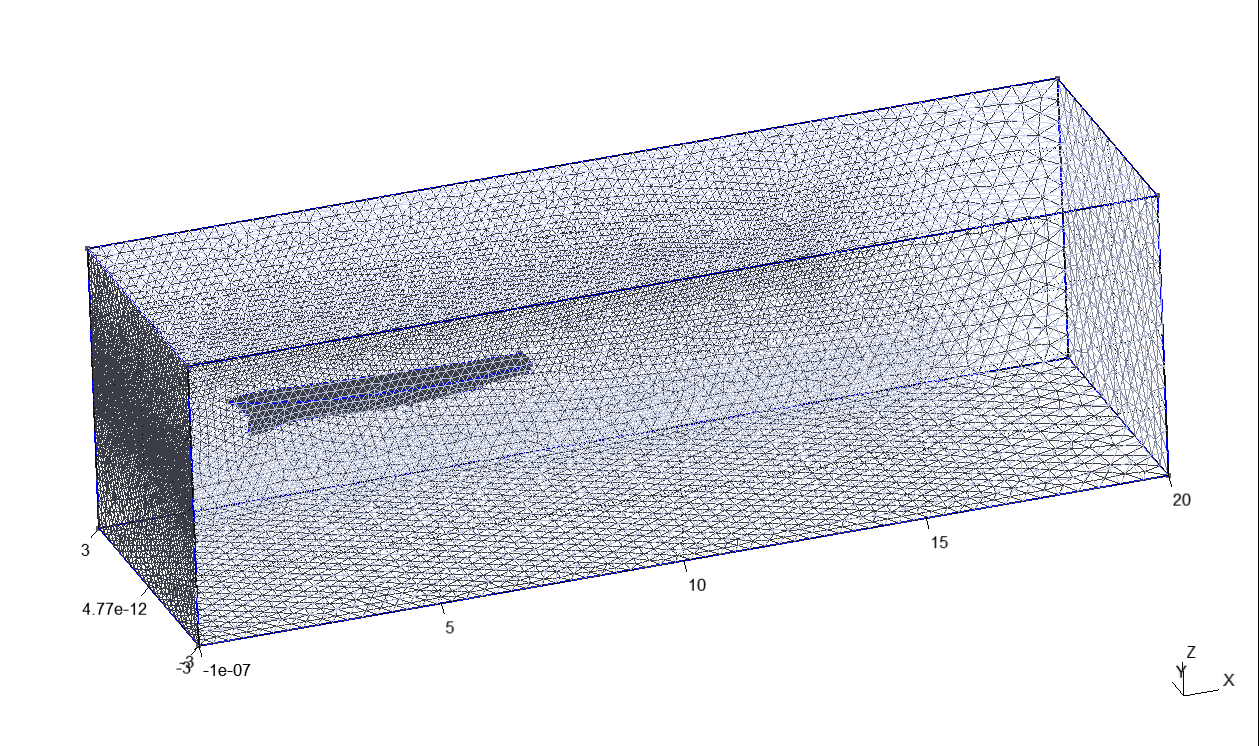
\includegraphics[width=1\textwidth]{Mesh_1.png}
    \caption{Mesh of the Domain}
    
\end{figure}
\begin{figure}[ht]
    \centering
    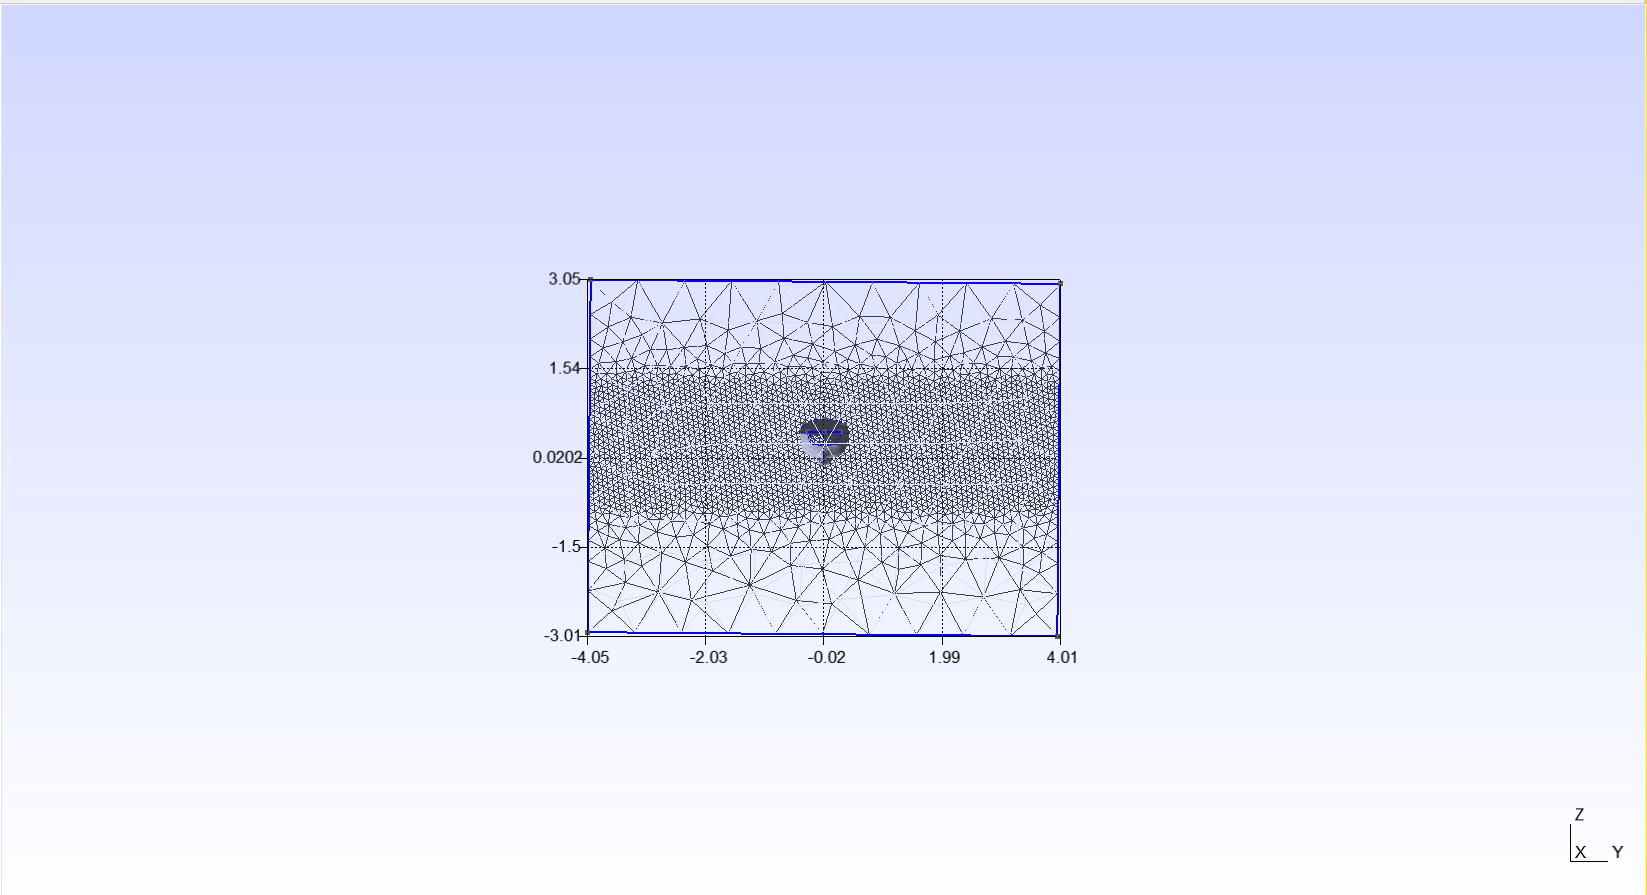
\includegraphics[width=1\textwidth]{Mesh_2.png}
    \caption{Front View of the Mesh}
\end{figure}

\begin{figure}[ht]
    \centering
    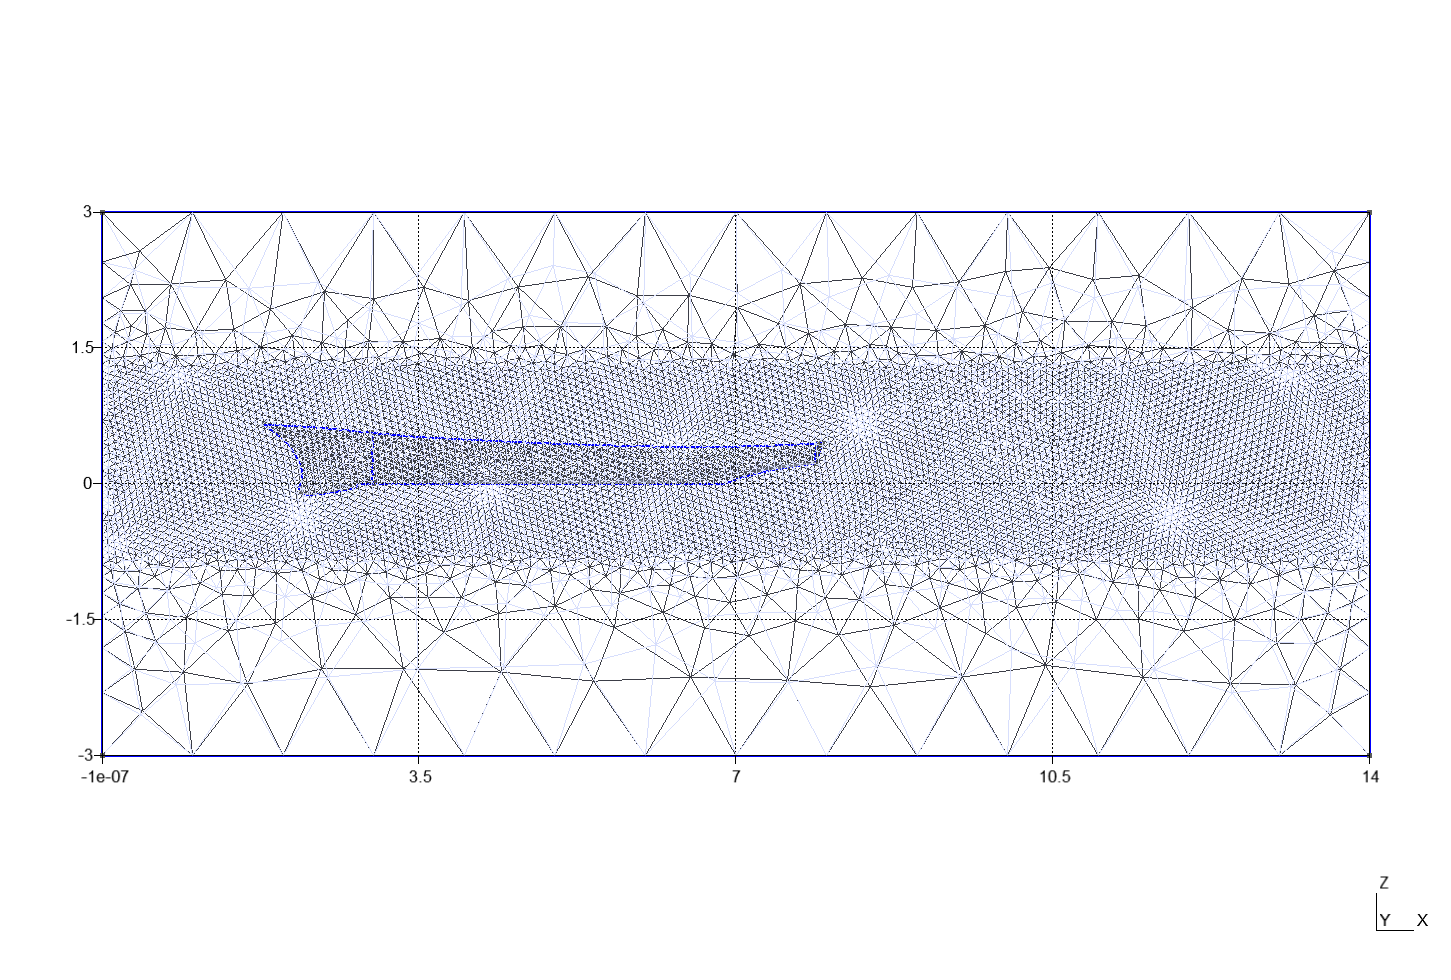
\includegraphics[width=1\textwidth]{Mesh_3.png}
    \caption{Side View of the Mesh}
\end{figure}

\begin{figure}[ht]
    \centering
    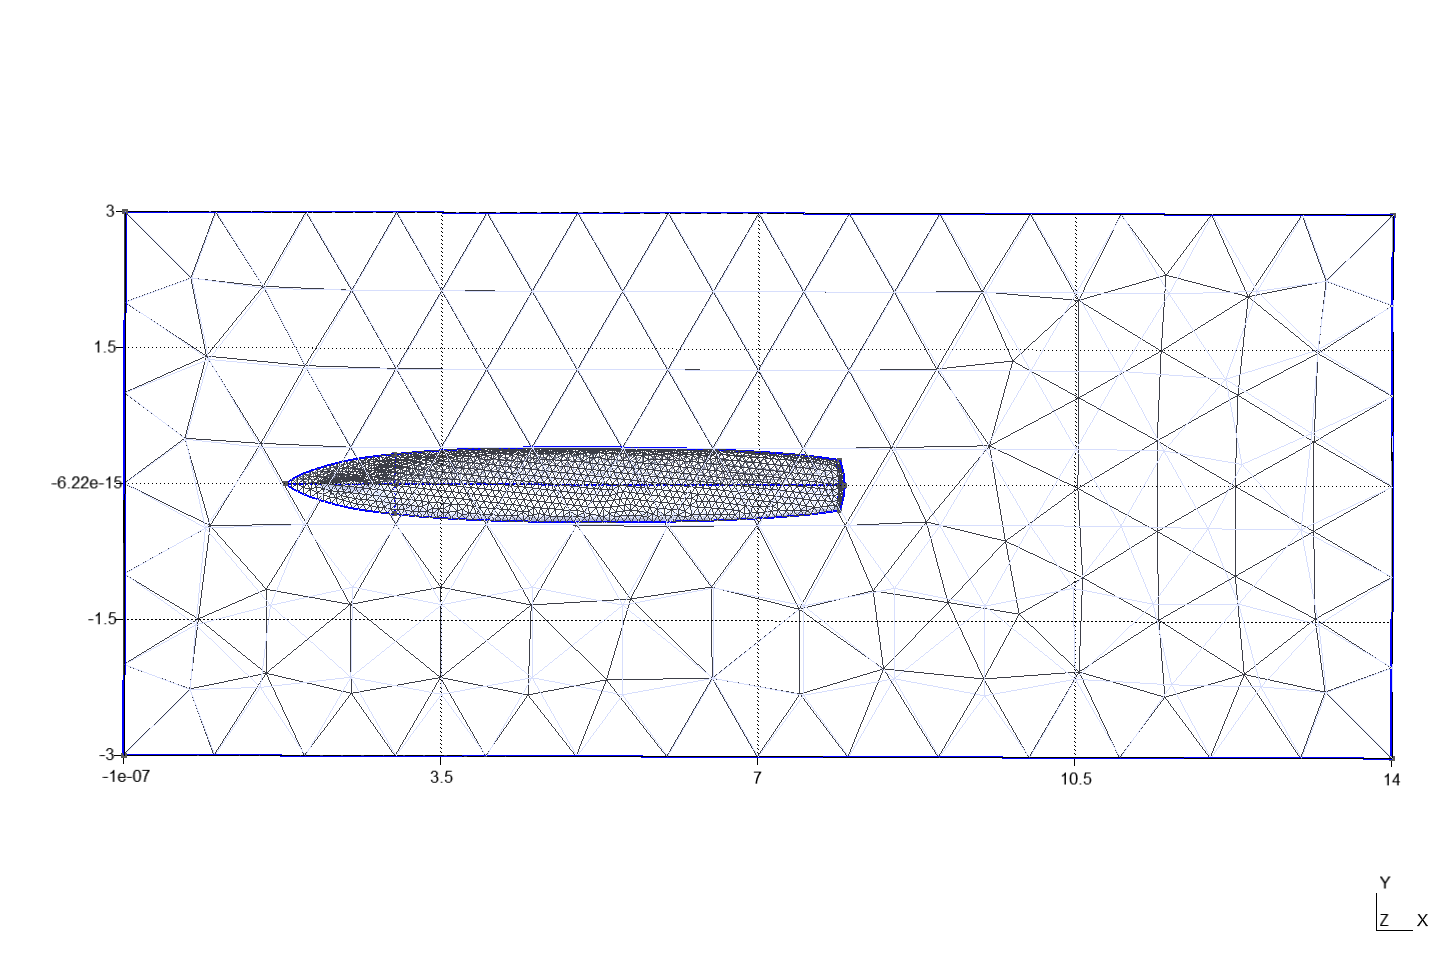
\includegraphics[width=1\textwidth]{Mesh_4.png}
    \caption{Top View of the Mesh}
\end{figure}
\clearpage
\subsection{Mesh Statistics}
\begin{figure}[ht]
    \centering
    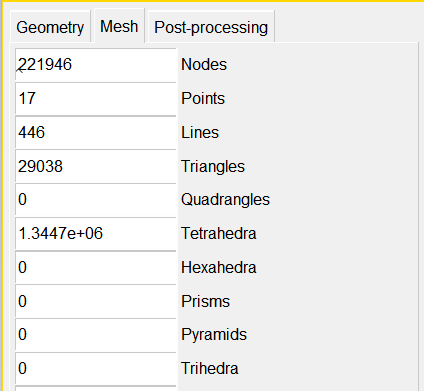
\includegraphics[width=0.5\textwidth]{MS.png}
    \caption{Mesh Statistics}
\end{figure}
\subsection{Wave Configuration}
\begin{table}[ht]
    \caption{Wave Conditions}
    \centering
    \begin{tabular}{|c|c|c|}
        \hline
        Parameters & Value & Unit\\
        \hline   
        $H_w$ & 0.32032 & m \\
        $k_w$ & 1.0845 & m\\
        $\lambda_w$ & 0.91 & m\\
        $T_w$ & 1.929 & m \\
        \hline
    \end{tabular}
\end{table}


\section{Result}

\section{Discussion}

\section{Conclusion}



\section{Reference}
\begin{thebibliography}{99}
    \bibitem{joshi2018}
    Vaibhav Joshi, \emph{Variational Methods and Applications for Turbulent Single and Two-Phase Fluid-Structure Interaction}, ScholarBank@NUS Repository, 2018.
\end{thebibliography}

\section{Appendix}
\subsection{DTMB 5415 Specifications}
\begin{table}[h!]
    \centering
    \begin{tabular}{|c|c|c|c|c|c|}
        \hline
        & \textbf{Full-Scale} & \textbf{\textcolor{blue}{MARIN}} & \textbf{\textcolor{blue}{INSEAN}} & \textbf{\textcolor{blue}{IIHR}} &\\ \hline
        \textbf{\textcolor{blue}{Lpp (m)}} & 142.00 & 4.002 & 4.002 & 5.719 & 3.048 \\ \hline
        \textbf{\textcolor{blue}{Lwl (m)}} & 142.18 & 4.007 & 4.008 & 5.726 & 3.052 \\ \hline
        \textbf{\textcolor{blue}{Bwl (m)}} & 19.06 & 0.537 & \textcolor{green}{0.538} & 0.768 & 0.409 \\ \hline
        \textbf{\textcolor{blue}{T (m)}} & 6.15 & 0.173 & \textcolor{green}{0.172} & 0.248 & 0.132 \\ \hline
        \textbf{\textcolor{blue}{Displacement (m\(^3\))}} & 8424.4 & 0.189 & \textcolor{green}{0.188} & 0.554 & 0.0826 \\ \hline
        \textbf{\textcolor{blue}{S w/o rudder (m\(^2\))}} & 2972.6 & 2.361 & \textcolor{green}{2.424} & TBD & TBD \\ \hline
        \textbf{\textcolor{blue}{CB}} & 0.507 & 0.507 & 0.507 & 0.506 & TBD \\ \hline
        \textbf{\textcolor{blue}{CM}} & 0.821 & 0.821 & 0.821 & 0.821 & 0.821 \\ \hline
        \textbf{\textcolor{blue}{LCB (\%Lpp), fwd+}} & -0.683 & -0.683 & \textcolor{green}{-0.652} & \textcolor{green}{-0.652} & TBD \\ \hline
    \end{tabular}
    \caption{Main particulars of the ship model}
\end{table}
\subsection{3D Mesh}
\begin{figure}[ht]
    \centering
    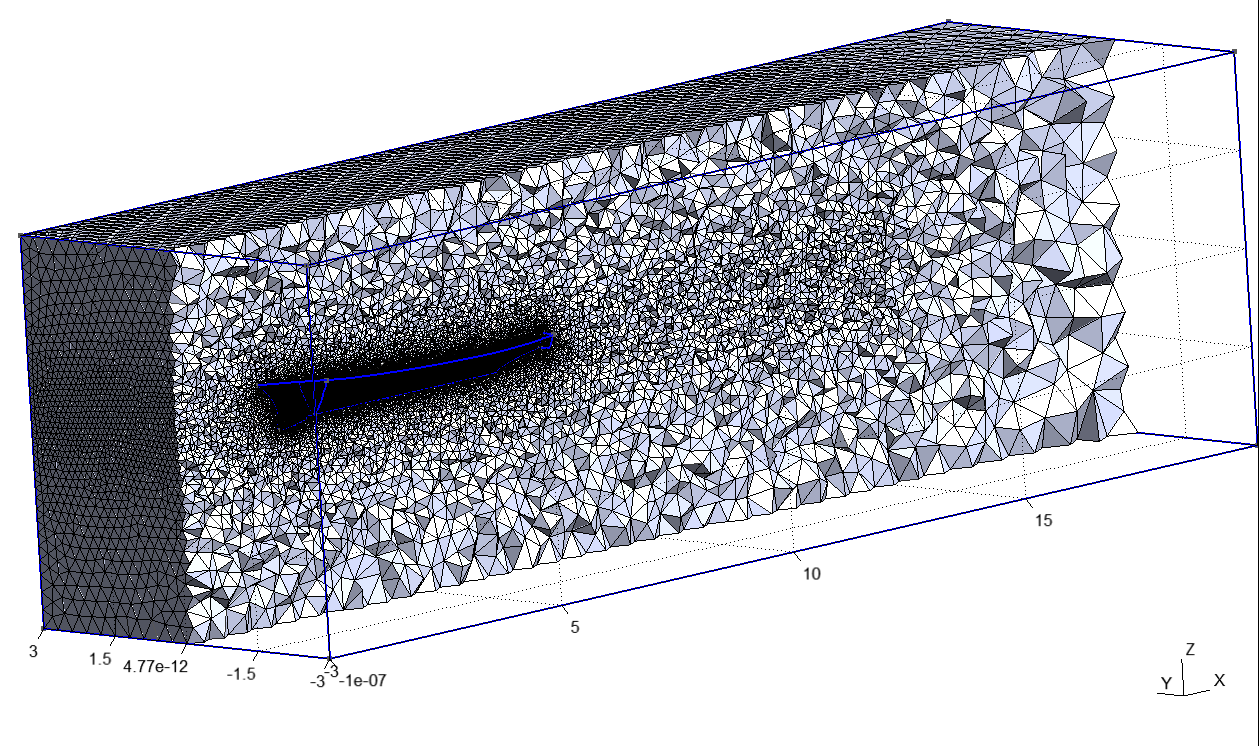
\includegraphics[width=1\textwidth]{Mesh_3D.png}
    \caption{3D Mesh}
\end{figure}

\end{document}